\usepackage{pdfpages}

\textbf{/F10/} \\
\textbf{Prozess:} Erstmaliges Öffnen der App \\
\textbf{Ziel:} Anlegen eines neuen Benutzernamens \\
\textbf{Kategorie:} primär \\
\textbf{Vorbedingung:} Download und Installation der App \\
\textbf{Nachbedingung (Erfolg):} Ein Benutzername ist festgelegt \\
\textbf{Nachbedingung (Fehlschlag):} Kein Benutzername ist festgelegt,\\
\textbf{Akteure:} Benutzer der App \\
\textbf{Auslösendes Ereignis:} Starten der App\\
\textbf{Beschreibung:} \\
1. App installieren \\
2. App starten       \\
3. Benutzername eingeben \\
4. Benutzername wird an Server weitergegeben \\
5. Ansicht wechselt zum Gruppenmenü \\
\textbf{Erweiterung:} \\
5.a) Ansicht wechselt zur Hauptansicht\\
\textbf{Alternativen:} \\

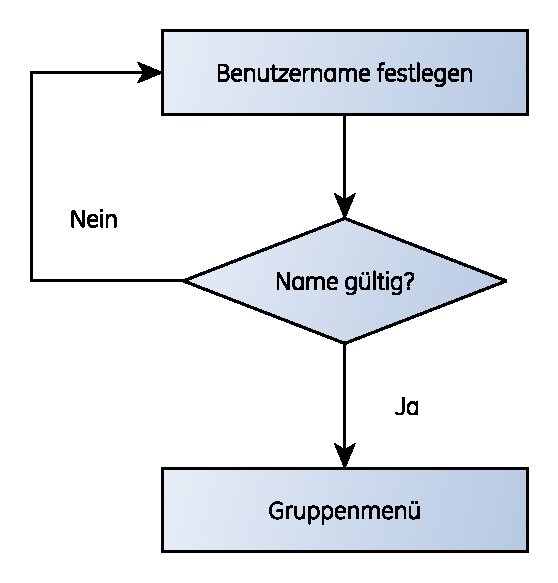
\includegraphics[scale=0.8]{erstmaliges-starten.pdf}
